\documentclass[11pt]{article} % use larger type; default would be 10pt

\usepackage{tikz}
\usetikzlibrary{calc}

        \newcommand\degree[0]{^{\circ}}

\title{Play with TikZ}
\author{Just Us}
%\date{} % Activate to display a given date or no date (if empty),
         % otherwise the current date is printed 

\begin{document}
\maketitle

\section{Angles}

%
1.1 Angles and Triangles


%%%%%%%%%%%%%
\begin{tikzpicture}

\filldraw[black] (0,0) circle (2pt) ;
\draw[blue, thick] (0,0)rectangle (.25,.25);
\draw [very thick, -> ] (0,0) -- (2,0);
\draw[very thick, black!50!blue,->] (0,0) -- (0,2);
\draw[red, thick, ->] (0.6,0) arc (0:90:.6) node [above right, midway] {$90 \degree$};


\filldraw[black] (5,0) circle (2pt);
%\draw[blue, thick] (5,0)rectangle (5.25,.25);
\draw [very thick, -> ] (5,0) -- (7,0);
\draw[very thick,black!50!blue, ->] (5,0) -- (3,0);
\draw[red, thick, ->] (5.5,0) arc (0:180:.5) node [above , midway] {$180 \degree$};


\filldraw[black] (8,0) circle (2pt);
\draw[blue, thick] (8,0)rectangle (8.25,-.25);
\draw [very thick, -> ] (8,0) -- (10,0);
\draw[very thick,black!50!blue, ->] (8,0) -- (8,-2);
\draw[red, thick, ->] (8.4,0) arc (0:270:.4) node [above left, midway] {$270 \degree$};


\filldraw[black] (11,0) circle (2pt);
%\draw[blue, thick] (5,0)rectangle (5.25,.25);
\draw [very thick, -> ] (11,0) -- (13,0);
\draw[very thick,black!50!blue, ->] (11,0) -- (13.2,0);
\draw[red, thick, ->] (11.4,0) arc (0:360:.4) node [below right] {$360 \degree$};

\end{tikzpicture}
\\
\section{Triangles}

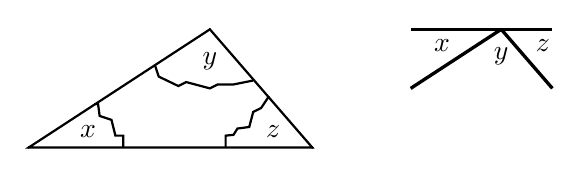
\begin{tikzpicture}
\filldraw[black] (0,0) circle (.2pt) node[anchor=south west, xshift=15] {$x$};
\filldraw[black] (3.6,0) circle (.2pt) node[anchor=south east, xshift=-8]{$z$};
\filldraw[black] (2.3,1.5) circle (.2pt) node[anchor=north, yshift=-5]{$y$};
\draw[black,  thick] (0,0) -- (3.6,0) -- (2.3,1.5) -- cycle;

\filldraw[black] (6,1.5) circle (.2pt) node[anchor=north east, xshift=-15] {$x$};
\filldraw[black] (6,1.5) circle (.2pt) node[anchor=north, yshift=-3] {$y$};
\filldraw[black] (6,1.5) circle (.2pt) node[anchor=north west, xshift=9] {$z$};
\draw[black,  very thick] (6,1.5) -- (4.85,1.5);
\draw[black,  very thick] (6,1.5) -- (4.85,0.75);
\draw[black,  very thick] (6,1.5) -- (6.65,0.75);
\draw[black,  very thick] (6,1.5) -- (6.65,1.5);

\draw[black, thick] (1.2,0) -- (1.2,.15) -- (1.1,.15) -- (1.05,.35) -- (.9,.4) -- (.88, .55)
-- (.83,.55);
\draw[black, thick] (2.5,0) -- (2.5,.15) -- (2.6,.16)--(2.65,.24)--(2.8,.26)--(2.85,.45)--(2.95, .5)
--(3.05,.65);
\draw[black, thick] (1.6,1.05)--(1.65,.9) -- (1.9,.78) --(2,.83) -- (2.3,.75) -- (2.4,.8)--(2.6,.8)
--(2.85,.85);
%\draw[green, ultra thick, dashed] (1.2,1) -- (1.2,-0.3);
%\draw[green, ultra thick, dashed] (2.9,1) -- (2.9,-0.3);
%\draw[green, ultra thick, dashdotted] (1,.8) -- (3.2,.8);

\end{tikzpicture}
\break
\newline

Example 1
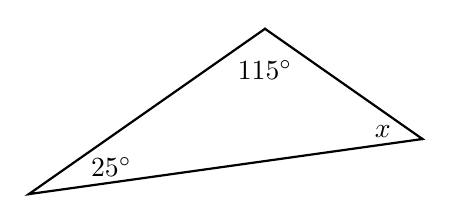
\begin{tikzpicture}
\coordinate (A) at (0,0);
\coordinate (B) at (5,0.7);
\coordinate(C) at (3,2.1);
\filldraw[black] (A) circle (.2pt) node[anchor=south west, xshift=19, yshift=3] {$25\degree$};
\filldraw[black] (B) circle (.2pt) node[anchor=south east, xshift=-8, yshift=-3] {$x$};
\filldraw[black] (C) circle (.2pt) node[anchor=north, yshift=-8] {$115\degree$};
\draw[black,  thick] (A) -- (B) --( C) -- cycle;
\end{tikzpicture}
\newline

Exercise 1
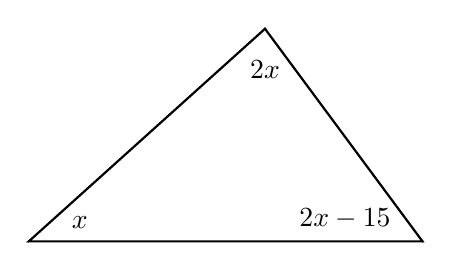
\begin{tikzpicture}
\coordinate (A) at (0,0);
\coordinate (B) at (5,0);
\coordinate(C) at (3,2.7);
\filldraw[black] (A) circle (.2pt) node[anchor=south west, xshift=12, yshift=1] {$x$};
\filldraw[black] (B) circle (.2pt) node[anchor=south east, xshift=-8, yshift=1] {$2x-15$};
\filldraw[black] (C) circle (.2pt) node[anchor=north, yshift=-8]{$2x$};
\draw[black,  thick] (A) -- (B) --( C) -- cycle;
\end{tikzpicture}
\newline

Example 2
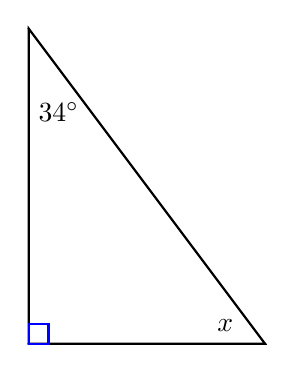
\begin{tikzpicture}
\coordinate (A) at (0,0);
\coordinate (B) at (3,0);
\coordinate(C) at (0,4);
\filldraw[black] (A) circle (.2pt) node[anchor=south west, xshift=10, yshift=1]{};
\filldraw[black] (B) circle (.2pt) node[anchor=south east, xshift=-8, yshift=1]{$x$};
\filldraw[black] (C) circle (.2pt) node[anchor=north west, yshift=-23]{$34\degree$};
\draw[black,  thick] (A) -- (B) --( C) -- cycle;
\draw[blue, thick] (0,0)rectangle (.25,.25);
\end{tikzpicture}
\newline

Example 3
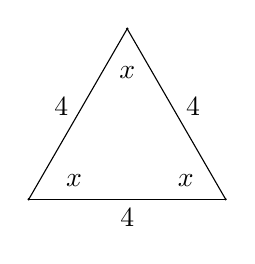
\begin{tikzpicture}
\coordinate (A) at (0,0);
\coordinate (B) at (2.5,0);
\coordinate(C) at (1.25,2.165);
\filldraw[black] (A) circle (.2pt) node[anchor=south west, xshift=10, yshift=1]{$x$};
\filldraw[black] (B) circle (.2pt) node[anchor=south east, xshift=-8, yshift=1]{$x$};
\filldraw[black] (C) circle (.2pt) node[anchor=north , yshift=-10]{$x$};
%\draw[black,  thick] (A) -- (B) --( C) -- cycle;
\draw[black] (A) --  (B) node [below, midway] {$4$};
\draw[black] (A) --  (C) node [above left, midway,yshift=-4] {$4$};
\draw[black] (C) --  (B) node [above right, midway,yshift=-4] {$4$};
\end{tikzpicture}
\newline


Exercise 3
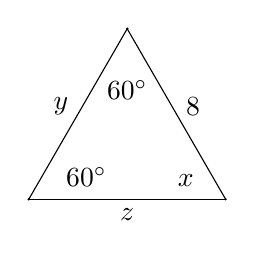
\begin{tikzpicture}
\coordinate (A) at (0,0);
\coordinate (B) at (2.5,0);
\coordinate(C) at (1.25,2.165);
\filldraw[black] (A) circle (.2pt) node[anchor=south west, xshift=10, yshift=1]{$60\degree$};
\filldraw[black] (B) circle (.2pt) node[anchor=south east, xshift=-8, yshift=1]{$x$};
\filldraw[black] (C) circle (.2pt) node[anchor=north , yshift=-15]{$60\degree$};
%\draw[black,  thick] (A) -- (B) --( C) -- cycle;
\draw[black] (A) --  (B) node [below, midway] {$z$};
\draw[black] (A) --  (C) node [above left, midway,yshift=-4] {$y$};
\draw[black] (C) --  (B) node [above right, midway,yshift=-4] {$8$};
\end{tikzpicture}
\newline


Example 4
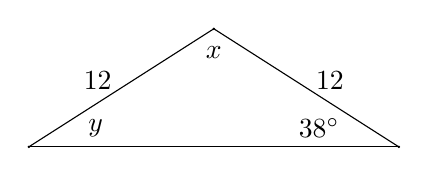
\begin{tikzpicture}
\coordinate (A) at (0,0);
\coordinate (B) at (4.7,0);
\coordinate(C) at (2.35,1.5);
\filldraw[black] (A) circle (.2pt) node[anchor=south west, xshift=18]{$y$};
\filldraw[black] (B) circle (.2pt) node[anchor=south east, xshift=-18]{$38\degree$};
\filldraw[black] (C) circle (.2pt) node[anchor=north , yshift=-3]{$x$};
%\draw[black,  thick] (A) -- (B) --( C) -- cycle;
\draw[black] (A) --  (B) node [below, midway] {};
\draw[black] (A) --  (C) node [above left, midway,yshift=-4] {$12$};
\draw[black] (C) --  (B) node [above right, midway,yshift=-4] {$12$};
\end{tikzpicture}
\newline

Exercise 4
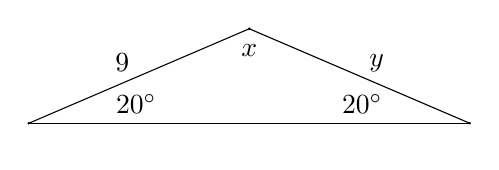
\begin{tikzpicture}
\coordinate (A) at (0,0);
\coordinate (B) at (5.6,0);
\coordinate(C) at (2.8,1.2);
\filldraw[black] (A) circle (.2pt) node[anchor=south west, xshift=28]{$20\degree$};
\filldraw[black] (B) circle (.2pt) node[anchor=south east, xshift=-28]{$20\degree$};
\filldraw[black] (C) circle (.2pt) node[anchor=north , yshift=-2]{$x$};
%\draw[black,  thick] (A) -- (B) --( C) -- cycle;
\draw[black] (A) --  (B) node [below, midway] {};
\draw[black] (A) --  (C) node [above left, midway,yshift=-2] {$9$};
\draw[black] (C) --  (B) node [above right, midway,yshift=-2] {$y$};
\end{tikzpicture}
\newline

Types of angles

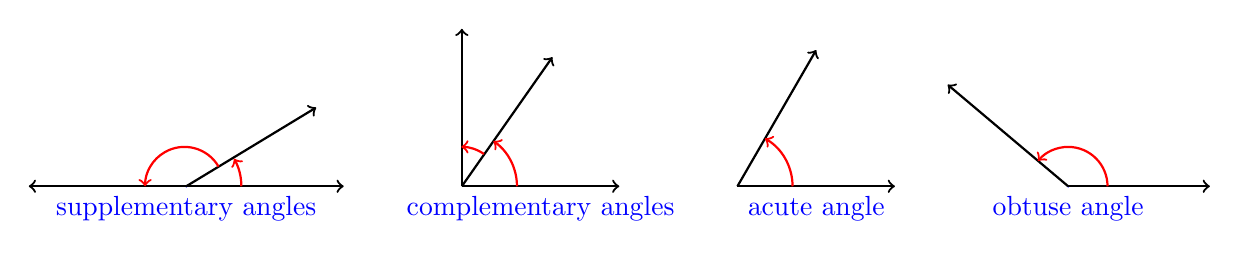
\begin{tikzpicture}

%supplementary
\coordinate (O) at (0,0);
\coordinate (A) at (-2,0);
\coordinate (B) at (2,0);
\coordinate(C) at (1.65,1);

\filldraw[blue] (O) circle (.2pt) node[anchor=north]{supplementary angles};

\draw[black, thick, <->] (A)--(B); 
\draw[black, thick, ->] (O)--(C); 
\draw[red, thick, ->] (.7,0) arc (0:30:.7);
\draw[red, thick, ->] (.41,.25) arc (30:180:.5);

%complementary
\coordinate (O2) at (3.5,0);
\coordinate (A2) at (5.5,0);
\coordinate (B2) at (3.5,2);
\coordinate(C2) at (4.65,1.64);

%\filldraw[blue] (O) circle (.2pt) node[anchor=north]{complementary angles};

\draw[black, thick, ->] (O2)--(A2)  node[below,midway ]{\color{blue}complementary angles}; 
\draw[black, thick, ->] (O2)--(B2); 
\draw[black, thick, ->] (O2)--(C2); 
\draw[red, thick, ->] (4.2,0) arc (0:55:.7);
\draw[red, thick, ->] (3.78,.41) arc (55:90:.5);

%acute
\coordinate (O3) at (7,0);
\coordinate (A3) at (9,0);
\coordinate (B3) at (8,1.73);

%\filldraw[blue] (O) circle (.2pt) node[anchor=north]{complementary angles};

\draw[black, thick, ->] (O3)--(A3)  node[below,midway ]{\color{blue}acute angle}; 
\draw[black, thick, ->] (O3)--(B3); 
\draw[red, thick, ->] (7.7,0) arc (0:60:.7);

%obtuse
\coordinate (O4) at (11.2,0);
\coordinate (A4) at (13.,0);
\coordinate (B4) at (9.67,1.29);

\filldraw[blue] (O4) circle (.2pt) node[anchor=north]{obtuse angle};

\draw[black, thick, ->] (O4)--(A4); 
\draw[black, thick, ->] (O4)--(B4); 
\draw[red, thick, ->] (11.7,0) arc (0:140:.5);

\end{tikzpicture}
\newline


Exercise 10
\begin{tikzpicture}
\coordinate (O) at (0,0);
\coordinate (A) at (-2,0);
\coordinate (B) at (2,0);
\coordinate(C) at (-1.157,-1.3789);
\coordinate (D) at (1.157,1.3789);
\filldraw[black] (O) circle (.2pt) node[anchor=south east]{$\alpha$};
\filldraw[black] (O) circle (.2pt) node[anchor=north east, xshift=-10]{$\beta$};
\filldraw[black] (O) circle (.2pt) node[anchor=north west, yshift=-2]{$\gamma$};
\filldraw[black] (O) circle (.2pt) node[anchor=south west, xshift=9]{$50\degree$};
\draw[black] (A) --  (B);
\draw[black] (C) --  (D) ;
\end{tikzpicture}
\newline



Example 1.9
\begin{tikzpicture}
\coordinate (O) at (0,0);
\coordinate (A) at (-2,0);
\coordinate (B) at (2,0);
\coordinate(C) at (.7,1.2);
\coordinate (D) at (0,-1.7);
\coordinate(E) at (1.8,-.5);
\draw[blue, thick] (O)rectangle (-.25,-.25);
\filldraw[black] (O) circle (.2pt) node[anchor=south east]{$O$};
\filldraw[black] (A) circle (.2pt) node[anchor=east]{$A$};
\filldraw[black] (B) circle (.2pt) node[anchor=west]{$B$};
\filldraw[black] (C) circle (.2pt) node[anchor=south west]{$C$};
\filldraw[black] (D) circle (.2pt) node[anchor=north west]{$D$};
\filldraw[black] (E) circle (.2pt) node[anchor=north west]{$E$};
%\draw[black,  thick] (A) -- (B) --( C) -- cycle;
\draw[black] (A) --  (O) --  (B);
\draw[black] (O) --  (C) ;
\draw[black] (O) --  (D) ;
\draw[black] (O) --  (E) ;
\end{tikzpicture}
\newline


Example 1.11
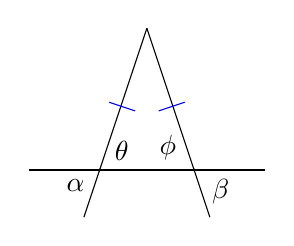
\begin{tikzpicture}
\coordinate (A) at (-.6,0);
\coordinate (B) at (0.6,0);
\coordinate(C) at (-.6,0);
\coordinate (D) at (0.6,0);
\filldraw[black] (A) circle (.2pt) node[anchor=south west, xshift=2]{$\theta$};
\filldraw[black] (B) circle (.2pt) node[anchor=south east, xshift=-3]{$\phi$};
\filldraw[black] (C) circle (.2pt) node[anchor=north east, xshift=-2]{$\alpha$};
\filldraw[black] (D) circle (.2pt) node[anchor=north west, xshift=3]{$\beta$};
\draw[black,  thick] (-1.5,0) -- (1.5,0);
\draw[black] (-.8,-.6) --  (0,1.8);
\draw[black] (0.8,-0.6) --  (0,1.8) ;
\draw[blue] (-.48,.86) -- (-.15,.75);
\draw[blue] (.48,.86) -- (.15,.75);

\end{tikzpicture}
\newline




Exercise 1.12
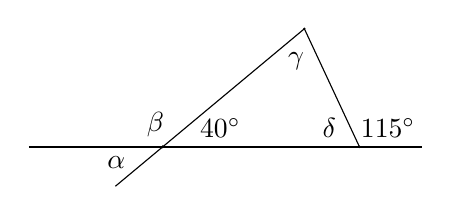
\begin{tikzpicture}
\coordinate (A) at (-1.8,0);
\coordinate (B) at (0.7,0);
\coordinate (C) at (0,1.50);
\filldraw[black] (A) circle (.2pt) node[anchor=south east, xshift=4]{$\beta$};
\filldraw[black] (A) circle (.2pt) node[anchor=south west, xshift=10]{$40\degree$};
\filldraw[black] (B) circle (.2pt) node[anchor=south east, xshift=-5]{$\delta$};
\filldraw[black] (A) circle (.2pt) node[anchor=north east, xshift=-10]{$\alpha$};
\filldraw[black] (B) circle (.2pt) node[anchor=south west, xshift=-3]{$115\degree$};
\filldraw[black] (C) circle (.2pt) node[anchor=north,xshift=-3, yshift=-5]{$\gamma$};
\draw[black,  thick] (-3.5,0) -- (1.5,0);
\draw[black] (-2.4,-.5) --  (0,1.5);
\draw[black] (B) --  (0,1.5) ;

\end{tikzpicture}
\newline



Parallel lines and transversal
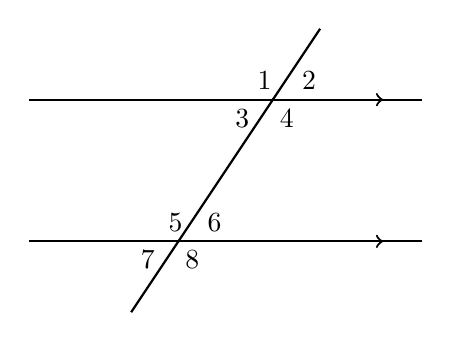
\begin{tikzpicture}
\coordinate (A) at (.6,1.8);
\coordinate (B) at (-.6,0);
\filldraw[black] (A) circle (.2pt) node[anchor=south east, xshift=3]{$1$};
\filldraw[black] (A) circle (.2pt) node[anchor=south west, xshift=7]{$2$};
\filldraw[black] (A) circle (.2pt) node[anchor=north east, xshift=-5]{$3$};
\filldraw[black] (A) circle (.2pt) node[anchor=north west, xshift=-1]{$4$};
\filldraw[black] (B) circle (.2pt) node[anchor=south east, xshift=5]{$5$};
\filldraw[black] (B) circle (.2pt) node[anchor=south west, xshift=7]{$6$};
\filldraw[black] (B) circle (.2pt) node[anchor=north east, xshift=-5]{$7$};
\filldraw[black] (B) circle (.2pt) node[anchor=north west, xshift=-1]{$8$};
\draw[black,  thick] (-2.5,1.8) -- (2.5,1.8);
\draw[black,  thick] (-2.5,0) -- (2.5,0);
\draw[black,  thick, ->] (-2.5,1.8) -- (2.,1.8);
\draw[black,  thick, ->] (-2.5,0) -- (2.,0);
\draw[black, thick] (-1.2,-.9) --  (1.2,2.7) ;

\end{tikzpicture}
\newline




Parallellogram
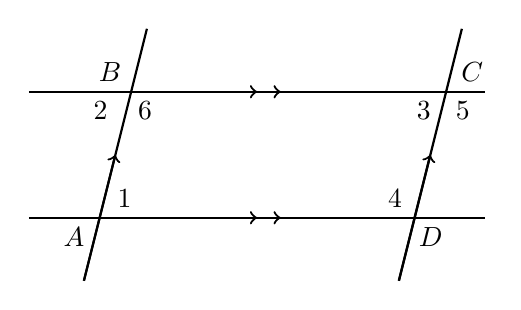
\begin{tikzpicture}
\coordinate (A) at (0,0);
\coordinate (B) at (.4,1.6);
\coordinate (C) at( 4.4,1.6);
\coordinate (D) at (4,0);
\filldraw[black] (A) circle (.2pt) node[anchor=north east, xshift=-2]{$A$};
\filldraw[black] (B) circle (.2pt) node[anchor=south east, xshift=0]{$B$};
\filldraw[black] (C) circle (.2pt) node[anchor=south west, xshift=2]{$C$};
\filldraw[black] (D) circle (.2pt) node[anchor=north west, xshift=-2]{$D$};
\filldraw[black] (D) circle (.2pt) node[anchor=south east, xshift=-1]{$4$};
\filldraw[black] (C) circle (.2pt) node[anchor=north east, xshift=-2]{$3$};
\filldraw[black] (C) circle (.2pt) node[anchor=north west, xshift=0]{$5$};
\filldraw[black] (A) circle (.2pt) node[anchor=south west, xshift=3]{$1$};
\filldraw[black] (B) circle (.2pt) node[anchor=north east, xshift=-5]{$2$};
\filldraw[black] (B) circle (.2pt) node[anchor=north west, xshift=-1]{$6$};
\draw[black,  thick] (-.9,1.6) -- (4.9,1.6);
\draw[black,  thick] (-.9,0) -- (4.9,0);
\draw[black,  thick, ->] (-.5,1.6) -- (2.,1.6);
\draw[black,  thick, ->] (-.5,0) -- (2.3,0);
\draw[black,  thick, ->] (-.5,1.6) -- (2.3,1.6);
\draw[black,  thick, ->] (-.5,0) -- (2.,0);
\draw[black, thick] (-.2,-.8) --  (.6,2.4) ;
\draw[black, thick] (3.8,-.8) --  (4.6,2.4) ;
\draw[black, thick, ->] (-.2,-.8) --  (.2,.8) ;
\draw[black, thick, ->] (3.8,-.8) --  (4.2,.8) ;
\end{tikzpicture}
\newline




Homework 1.1.1 answer
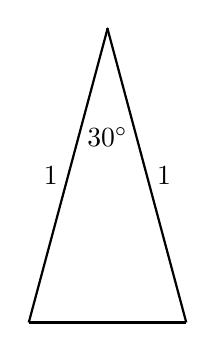
\begin{tikzpicture}
\coordinate (A) at (0,0);
\coordinate (B) at (2,0);
\coordinate (C) at (1,3.73);
\filldraw[black] (C) circle (.2pt) node[anchor=north , xshift=0,yshift=-32] {$30\degree$};

\draw[black, thick] (A)--(C)  node[left,midway ]{1}; 
\draw[black, thick] (B)--(C)  node[right,midway ]{1};
\draw[black, thick] (A)--(B); 

\end{tikzpicture}
\newline

Homework 1.1.3 answer
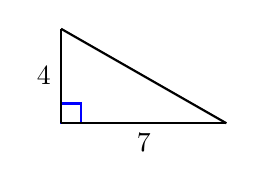
\begin{tikzpicture}
\coordinate (A) at (0,0);
\coordinate (B) at (2.1,0);
\coordinate (C) at (0,1.2);
\draw[blue, thick] (0,0) rectangle (.25,.25);

\draw[black, thick] (A)--(C)  node[left,midway ]{4}; 
\draw[black, thick] (B)--(C);
\draw[black, thick] (A)--(B)  node[below,midway ]{7}; 

\end{tikzpicture}
\newline

Homework 1.1.5 answer
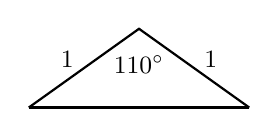
\begin{tikzpicture}
\coordinate (A) at (0,0);
\coordinate (B) at (1.4,-1);
\coordinate (C) at (-1.4,-1);

\draw[black, thick] (A)--(C)  node[left,midway, yshift=3 ]{\small 1}; 
\draw[black, thick] (B)--(C);
\draw[black, thick] (A)--(B)  node[right,midway,yshift=3 ]{\small1}; 
\filldraw[black] (A) circle (.2pt) node[anchor=north, yshift=-6] {\small$110\degree$};

\end{tikzpicture}
\newline

Homework 1.1.7
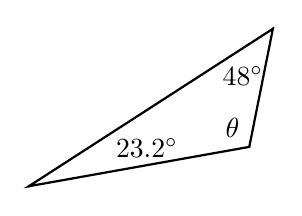
\begin{tikzpicture}
\coordinate (A) at (0,0);
\coordinate (B) at (2.8,.5);
\coordinate (C) at( 3.1,2.);
\filldraw[black] (A) circle (.2pt) node[anchor=south west, xshift=28, yshift=7] {$23.2\degree$};
\filldraw[black] (B) circle (.2pt) node[anchor=south east, xshift=0]{$\theta$};
\filldraw[black] (C) circle (.2pt) node[anchor=north east, xshift=0,yshift=-10] {$48\degree$};\draw[black,  thick] (A) -- (B) --( C) -- cycle;
\end{tikzpicture}
\newline



Homework 1.1.8
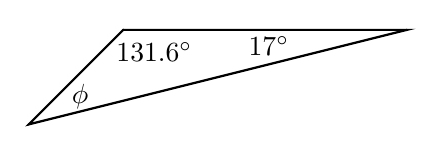
\begin{tikzpicture}
\coordinate (A) at (0,0);
\coordinate (B) at (4.8,1.2);
\coordinate (C) at( 1.2,1.2);
\filldraw[black] (A) circle (.2pt) node[anchor=south west, xshift=12, yshift=2] {$\phi$};
\filldraw[black] (B) circle (.2pt) node[anchor=north east, xshift=-39,yshift=1] {$17\degree$};
\filldraw[black] (C) circle (.2pt) node[anchor=north west, xshift=-6,yshift=-1] {$131.6\degree$};\draw[black,  thick] (A) -- (B) --( C) -- cycle;
\end{tikzpicture}
\newline



Homework 1.1.9
\begin{tikzpicture}
\coordinate (A) at (0,0);
\coordinate (B) at (3.7,0);
\coordinate (C) at( 0,-2);
%\filldraw[black] (A) circle (.2pt) node[anchor=south west, xshift=8, yshift=2]{$x$};
\filldraw[black] (B) circle (.2pt) node[anchor=north east, xshift=-15,yshift=1]{$\alpha$};
\filldraw[black] (C) circle (.2pt) node[anchor=south west, xshift=-0,yshift=6]{$61\degree$};\draw[black,  thick] (A) -- (B) --( C) -- cycle;
\draw[blue, thick] (O)rectangle (.25,-.25);
\end{tikzpicture}
\newline



Homework 1.1.10
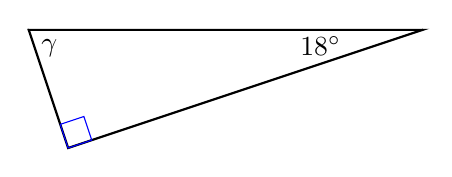
\begin{tikzpicture}
\coordinate (A) at (0,0);
\coordinate (B) at (5,0);
\coordinate (C) at( 0.5,-1.5);
\filldraw[black] (A) circle (.2pt) node[anchor=north west, xshift=1, yshift=0]{$\gamma$};
\filldraw[black] (B) circle (.2pt) node[anchor=north east, xshift=-26,yshift=1]{$18\degree$};
%\filldraw[black] (C) circle (.2pt) node[anchor=south west, xshift=-0,yshift=6](a) {$61\degree$};
\draw[black,  thick] (A) -- (B) --( C) -- cycle;
\draw[blue] (0.4,-1.2) -- (0.7,-1.1) --(0.8,-1.4) --( C)  -- cycle;
%\draw[blue, thick] (O)rectangle (.25,-.25);
\end{tikzpicture}
\newline


Homework 1.1.11
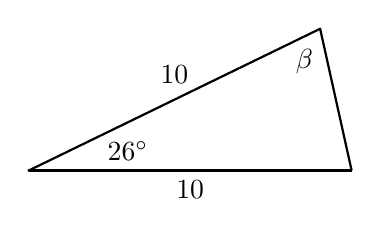
\begin{tikzpicture}
\coordinate (A) at (0,0);
\coordinate (B) at (4.1,0);
\coordinate (C) at( 3.7,1.8);
\filldraw[black] (A) circle (.2pt) node[anchor=south west, xshift=25, yshift=0]{$26\degree$};
\filldraw[black] (C) circle (.2pt) node[anchor=north east, xshift=1,yshift=-4]{$\beta$};
%\draw[black,  thick] (A) -- (B) --( C) -- cycle;
\draw[black,  thick] (A) --  (B) node [below, midway] {$10$};
\draw[black,  thick] (A) --  (C) node [above, midway, yshift=2] {$10$};
\draw[black,  thick] (B)--(C);
\end{tikzpicture}
\newline



Homework 1.1.12
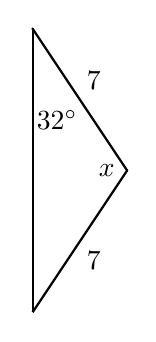
\begin{tikzpicture}
\coordinate (A) at (0,0);
\coordinate (B) at (1.2,1.8);
\coordinate (C) at( 0,3.6);
\filldraw[black] (B) circle (.2pt) node[anchor=east, xshift=-1, yshift=0]{$x$};
\filldraw[black] (C) circle (.2pt) node[anchor=north west, xshift=-2,yshift=-26]{$32\degree$};
%\draw[black,  thick] (A) -- (B) --( C) -- cycle;
\draw[black,  thick] (A) --  (B) node [below, midway, xshift=5] {$7$};
\draw[black,  thick] (B) --  (C) node [above, midway, xshift=5] {$7$};
\draw[black,  thick] (A)--(C);
\end{tikzpicture}
\newline



Homework 1.1.13
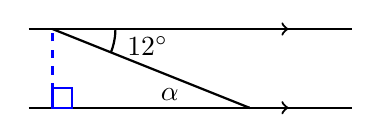
\begin{tikzpicture}
\coordinate (A) at (0,0);
\coordinate (B) at (2.5,0);
\coordinate (C) at( 0,1.);
\coordinate (D) at( 2.5,1.);
\filldraw[black] (B) circle (.2pt) node[anchor=south east, xshift=-22, yshift=-1]{$\alpha$};
\draw[black, thick] (.8,1) arc (0:-21.8:.8) node [right, midway, xshift=1, yshift=-2] {$12 \degree$};
\draw[black,  thick] (B) --( C);
\draw[black,  thick] (-.3,0) --  (3.8,0);
\draw[black,  thick] (-.3,1.) --  (3.8,1);
\draw[black,  thick,->] (-.3,0) --  (3,0);
\draw[black,  thick,->] (-.3,1.) --  (3,1.);
\draw[blue,  thick, dashed] (A)--(C);
\draw[blue, thick] (A) rectangle (.25,.25);
\end{tikzpicture}
\newline



Homework 1.1.14
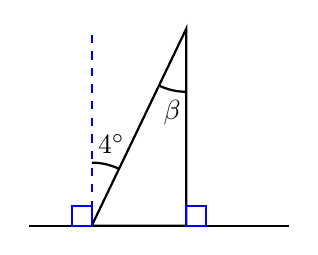
\begin{tikzpicture}
\coordinate (A) at (0,0);
\coordinate (B) at (1.2,0);
\coordinate (C) at( 1.2,2.5);
\coordinate (D) at( 0,2.5);
\draw[black, thick] (1.2,1.7) arc (-90:-115.64:.8) node [below, midway, xshift=0, yshift=0] {$\beta$};
%\filldraw[black] (C) circle (.2pt) node[anchor=north east, xshift=-2, yshift=-12]{$\beta$};
\draw[black, thick] (0,.8) arc (90:64.36:.8) node [above, midway, xshift=2, yshift=0] {$4 \degree$};
\draw[black,  thick] (A) -- (B) --(C) -- cycle;
\draw[black,  thick] (-.8,0) --  (2.5,0);
\draw[blue,  thick, dashed] (A)--(0,2.5);
\draw[blue, thick] (A) rectangle (-.25,.25);
\draw[blue, thick] (B) rectangle +(.25,.25);
\end{tikzpicture}
\newline



Homework 1.1.15
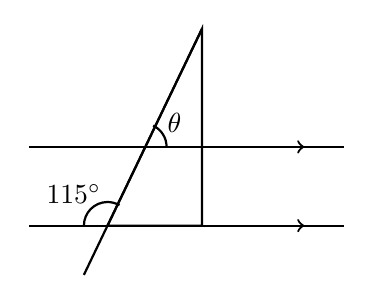
\begin{tikzpicture}
\coordinate (A) at (0,0);
\coordinate (B) at (1.2,0);
\coordinate (C) at( 1.2,2.5);

\draw[black, thick] (-.3,0) arc (180:59.6:.3) node [above, midway, xshift=-8, yshift=-3] {$115\degree$};
\draw[black, thick] (.75,1) arc (0:64.36:.3) node [above right, midway, xshift=-2, yshift=-3] {$\theta$};

\draw[black,  thick] (A)--(B) --( C) -- cycle;
\draw[black,  thick] (-.3,-.625) --( C);
\draw[black,  thick] (-1,0) --  (3.,0);
\draw[black,  thick] (-1,1.) --  (3.,1);
\draw[black,  thick,->] (B) --  (2.5,0);
\draw[black,  thick,->] (1.2,1) --  (2.5,1);

\end{tikzpicture}
\newline




Homework 1.1.16
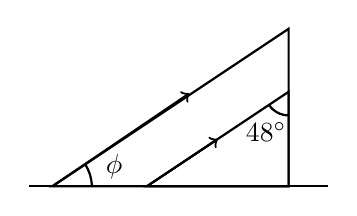
\begin{tikzpicture}
\coordinate (A) at (0,0);
\coordinate (B) at (0,1.2);
\coordinate (C) at(-1.8,0);
\coordinate (D) at (0,2);
\coordinate (E) at (-3,0);
\coordinate (F) at (-.9,.6);
\coordinate(G) at (-1.26,1.18);

\draw[black, thick] (0,.9) arc (-90:-147.3:.3) node [below left, midway, xshift=7, yshift=0] {$48\degree$};
\draw[black, thick] (-2.5,0) arc (0:34.3:.5) node [right, midway, xshift=2, yshift=3] {$\phi$};

\draw[black,  thick] (A)--(B) --( C) -- cycle;
\draw[black,  thick] (A)--(D) --( E) -- cycle;

%\draw[black,  thick] (-3.3,-.625) --(2,3);
\draw[black,  thick] (-3.3,0) --  (.5,0);
%\draw[black,  thick] (-1,1.) --  (3.,1);
\draw[black,  thick,->] (C) --  (F);
\draw[black,  thick,->] (E) --  (G);

\end{tikzpicture}
\newline




Homework 1.1.17
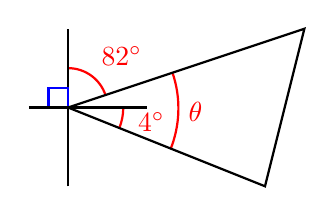
\begin{tikzpicture}
\coordinate (A) at (0,0);
\coordinate (B) at (2.5,-1);
\coordinate (C) at (3,1);

\draw[red, thick] (0,.5) arc (90:18.4:.5) node [above right, midway,xshift=0, yshift=0] {$82\degree$};
\draw[red, thick] (.7,0) arc (0:-21.8:.7) node [right, midway, xshift=2, yshift=-1.5] {$4\degree$};
\draw[red, thick] (1.3,-0.53) arc (-21.8:18.4:1.4) node [right, midway, xshift=0, yshift=0] {$\theta$};

\draw[black,  thick] (A)--(B) --( C) -- cycle;

\draw[black,  thick] (0,-1) --(0,1);
\draw[blue, thick] (A) rectangle (-.25,.25);
\draw[black,  thick] (-.5, 0) --  (1, 0);

\end{tikzpicture}
\newline


Homework 1.1.18
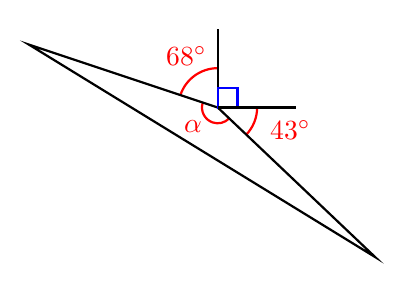
\begin{tikzpicture}
\coordinate (A) at (0,0);
\coordinate (B) at (2,-1.9);
\coordinate (C) at (-2.4,0.8);

\draw[red, thick] (0,.5) arc (90:161.6:.5) node [above , midway,xshift=-3, yshift=0] {$68\degree$};
\draw[red, thick] (.5,0) arc (0:-43.5:.5) node [right, midway, xshift=2, yshift=-3] {$43\degree$};
\draw[red, thick] (-.19,0.063) arc (161.6:316.5:.2) node [below, midway, xshift=-6, yshift=4] {$\alpha$};

\draw[black,  thick] (A)--(B) --( C) -- cycle;

\draw[black,  thick] (A) --(0,1);
\draw[blue, thick] (A) rectangle (.25,.25);
\draw[black,  thick] (A) --  (1, 0);

\end{tikzpicture}
\newline


Homework 1.1.19
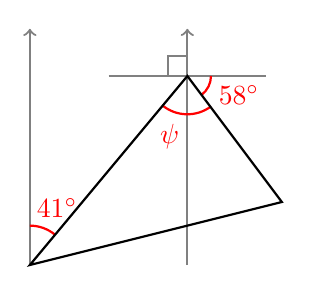
\begin{tikzpicture}
\coordinate (A) at (0,0);
\coordinate (B) at (3.2,0.8);
\coordinate (C) at (2,2.4);

\draw[gray,  thick,->] (A) --(0,3);
\draw[gray,  thick,->] (2,0) --(2,3);
\draw[gray, thick] (C) rectangle +(-.25,.25);
\draw[gray,  thick] (1,2.4) --  (3, 2.4);

\draw[red, thick] (0,.5) arc (90:50.2:.5) node [above , midway,xshift=5, yshift=0] {$41\degree$};
\draw[red, thick] (2.3,2.4) arc (0:-53.1:.3) node [right, midway, xshift=0, yshift=-3] {$58\degree$};
\draw[red, thick] (1.68,2.03) arc (230.2:306.9:.5) node [below, midway, xshift=-6, yshift=0] {$\psi$};

\draw[black,  thick] (A)--(B) --( C) -- cycle;

\end{tikzpicture}
\newline



Homework 1.1.20
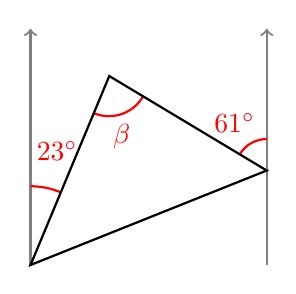
\begin{tikzpicture}
\coordinate (A) at (0,0);
\coordinate (B) at (1,2.4);
\coordinate (C) at (3,1.2);

\draw[gray,  thick,->] (A) --(0,3);
\draw[gray,  thick,->] (3,0) --(3,3);

\draw[red, thick] (0,1) arc (90:67.3:1) node [above , midway,xshift=4, yshift=6] {$23\degree$};
\draw[red, thick] (3,1.6) arc (90:149.1:.4) node [above left, midway, xshift=5, yshift=0] {$61\degree$};
\draw[red, thick] (0.8,1.93) arc (247:331:.5) node [below, midway, xshift=0, yshift=0] {$\beta$};

\draw[black,  thick] (A)--(B) --( C) -- cycle;

\end{tikzpicture}
\newline



Homework 1.1.21
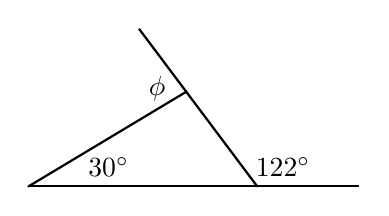
\begin{tikzpicture}
\coordinate (A) at (0,0);
\coordinate (B) at (2.9,0);
\coordinate (C) at( 2,1.2);
\filldraw[black] (A) circle (.2pt) node[anchor=south west, xshift=18, yshift=0]{$30\degree$};
\filldraw[black] (B) circle (.2pt) node[anchor=south west, xshift=-4, yshift=0]{$122\degree$};
\filldraw[black] (C) circle (.2pt) node[anchor=east, xshift=-4,yshift=1]{$\phi$};

\draw[black,  thick] (1.4,2) --  (B);
\draw[black,  thick] (A) --  (4.2,0);
\draw[black,  thick] (A)--(C);
\end{tikzpicture}
\newline



Homework 1.1.22
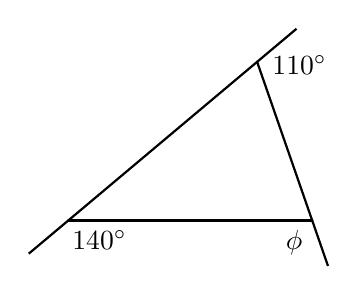
\begin{tikzpicture}
\coordinate (A) at (0,0);
\coordinate (B) at (3.1,0);
\coordinate (C) at( 2.4,2.016);
\filldraw[black] (A) circle (.2pt) node[anchor=north west, xshift=-2, yshift=0]{$140\degree$};
\filldraw[black] (B) circle (.2pt) node[anchor=north east, xshift=0, yshift=0]{$\phi$};
\filldraw[black] (C) circle (.2pt) node[anchor=west, xshift=2,yshift=-1]{$110\degree$};
%\draw[black,  thick] (A) -- (B) --( C) -- cycle;
\draw[black,  thick] (-.5,-.42) --  (2.9,2.436);
\draw[black,  thick] (C) --  (3.3,-.576);
\draw[black,  thick] (A)--(B);
\end{tikzpicture}
\newline


Homework 1.1.23A
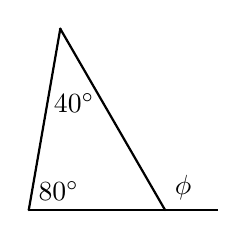
\begin{tikzpicture}
\coordinate (A) at (0,0);
\coordinate (B) at (1.73,0);
\coordinate (C) at( .4,2.3);
\filldraw[black] (A) circle (.2pt) node[anchor=south west, xshift=0, yshift=0]{$80\degree$};
\filldraw[black] (B) circle (.2pt) node[anchor=south west, xshift=0, yshift=0]{$\phi$};
\filldraw[black] (C) circle (.2pt) node[anchor=north, xshift=5,yshift=-20]{$40\degree$};

\draw[black,  thick] (B) --  (C);
\draw[black,  thick] (C) --  (A);
\draw[black,  thick] (A)--(2.4,0);
\end{tikzpicture}
\newline


Homework 1.1.23B
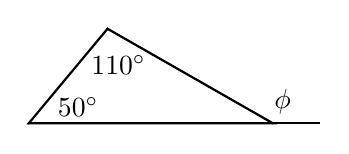
\begin{tikzpicture}
\coordinate (A) at (0,0);
\coordinate (B) at (3.1,0);
\coordinate (C) at(1,1.2);
\filldraw[black] (A) circle (.2pt) node[anchor=south west, xshift=7, yshift=-1]{$50\degree$};
\filldraw[black] (B) circle (.2pt) node[anchor=south west, xshift=-3, yshift=0]{$\phi$};
\filldraw[black] (C) circle (.2pt) node[anchor=north , xshift=4,yshift=-6]{$110\degree$};
\draw[black,  thick] (A) -- (B) --( C) -- cycle;
\draw[black,  thick] (A)--(3.7,0);
\end{tikzpicture}
\newline


Homework 1.1.23c
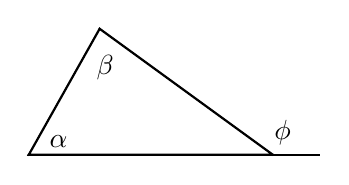
\begin{tikzpicture}
\coordinate (A) at (0,0);
\coordinate (B) at (3.1,0);
\coordinate (C) at(.9,1.6);
\filldraw[black] (A) circle (.2pt) node[anchor=south west, xshift=4, yshift=-1]{$\alpha$};
\filldraw[black] (B) circle (.2pt) node[anchor=south west, xshift=-3, yshift=0]{$\phi$};
\filldraw[black] (C) circle (.2pt) node[anchor=north , xshift=2,yshift=-6]{$\beta$};
\draw[black,  thick] (A) -- (B) --( C) -- cycle;
\draw[black,  thick] (A)--(3.7,0);
\end{tikzpicture}
\newline


Homework 1.1.24a
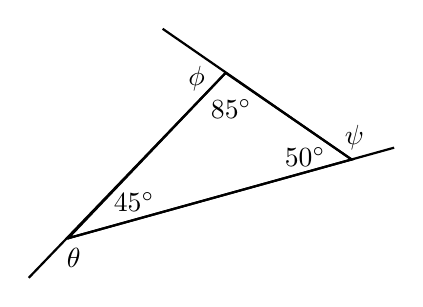
\begin{tikzpicture}
\coordinate (A) at (0,0);
\coordinate (B) at (3.6,1);
\coordinate (C) at(2,2.1);

\filldraw[black] (A) circle (.2pt) node[anchor=south west, xshift=13, yshift=6]{$45\degree$};
\filldraw[black] (B) circle (.2pt) node[anchor=east, xshift=-6, yshift=1]{$50\degree$};
\filldraw[black] (C) circle (.2pt) node[anchor=north , xshift=2,yshift=-6]{$85\degree$};

\filldraw[black] (A) circle (.2pt) node[anchor=north  west, xshift=-4, yshift=0]{$\theta$};
\filldraw[black] (B) circle (.2pt) node[anchor=south, xshift=1, yshift=0]{$\psi$};
\filldraw[black] (C) circle (.2pt) node[anchor=east , xshift=-4,yshift=-2]{$\phi$};

\draw[black,  thick] (A) -- (B) --( C) -- cycle;
\draw[black,  thick] (B) --  (1.2,2.66);
\draw[black,  thick] (C) --  (-.5,-.5025);
\draw[black,  thick] (A)--(4.14,1.15);
\end{tikzpicture}
\newline


Homework 1.1.24b
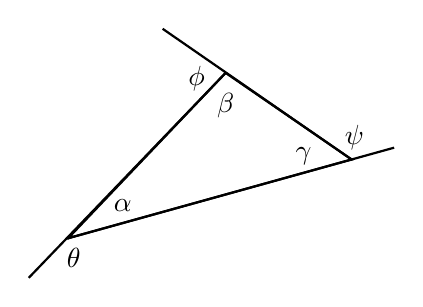
\begin{tikzpicture}
\coordinate (A) at (0,0);
\coordinate (B) at (3.6,1);
\coordinate (C) at(2,2.1);

\filldraw[black] (A) circle (.2pt) node[anchor=south west, xshift=13, yshift=6]{$\alpha$};
\filldraw[black] (B) circle (.2pt) node[anchor=east, xshift=-11, yshift=1]{$\gamma$};
\filldraw[black] (C) circle (.2pt) node[anchor=north , xshift=0,yshift=-4]{$\beta$};

\filldraw[black] (A) circle (.2pt) node[anchor=north  west, xshift=-4, yshift=0]{$\theta$};
\filldraw[black] (B) circle (.2pt) node[anchor=south, xshift=1, yshift=0]{$\psi$};
\filldraw[black] (C) circle (.2pt) node[anchor=east , xshift=-4,yshift=-2]{$\phi$};

\draw[black,  thick] (A) -- (B) --( C) -- cycle;
\draw[black,  thick] (B) --  (1.2,2.66);
\draw[black,  thick] (C) --  (-.5,-.5025);
\draw[black,  thick] (A)--(4.14,1.15);
\end{tikzpicture}
\newline


Homework 1.1.25
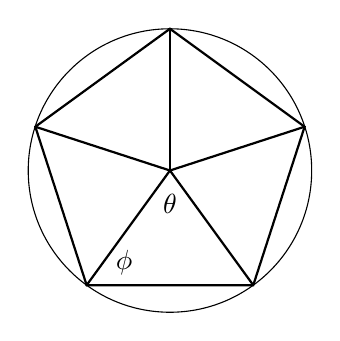
\begin{tikzpicture}
\coordinate(O) at (0,0);
\coordinate (A) at (1.71,.556 );
\coordinate (B) at (0,1.8);
\coordinate (C) at(-1.71,.556);
\coordinate (D) at (-1.058,-1.456);
\coordinate (E) at(1.058,-1.456);

\draw (0,0) circle (1.8);
\filldraw[black] (O) circle (.2pt) node[anchor=north, xshift=0, yshift=-5]{$\theta$};
\filldraw[black] (D) circle (.2pt) node[anchor=south west, xshift=7, yshift=0]{$\phi$};

\draw[black,  thick] (A) -- (B) --( C) --(D) --(E)-- cycle;
\draw[black,  thick] (B) --  (O);
\draw[black,  thick] (C) --  (O);
\draw[black,  thick] (A)--(O);
\draw[black,  thick] (D) --  (O);
\draw[black,  thick] (E)--(O);

\end{tikzpicture}
\newline


Homework 1.1.26
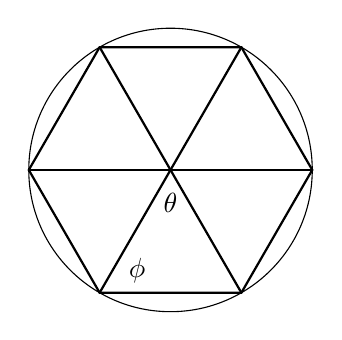
\begin{tikzpicture}
\coordinate(O) at (0,0);
\coordinate (A) at (1.8,0 );
\coordinate (B) at (0.9,1.559);
\coordinate (C) at(-.9,1.559);
\coordinate (D) at (-1.8,0);
\coordinate (E) at(-0.9,-1.559);
\coordinate (F) at(0.9,-1.559);

\draw (0,0) circle (1.8);
\filldraw[black] (O) circle (.2pt) node[anchor=north, xshift=0, yshift=-5]{$\theta$};
\filldraw[black] (E) circle (.2pt) node[anchor=south west, xshift=7, yshift=0]{$\phi$};

\draw[black,  thick] (A) -- (B) --( C) --(D) --(E)--(F) -- cycle;
\draw[black,  thick] (B) --  (O);
\draw[black,  thick] (C) --  (O);
\draw[black,  thick] (A)--(O);
\draw[black,  thick] (D) --  (O);
\draw[black,  thick] (E)--(O);
\draw[black,  thick] (F)--(O);

\end{tikzpicture}
\newline


Homework 1.1.27
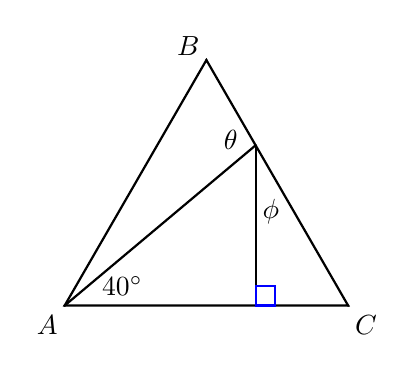
\begin{tikzpicture}
\coordinate (A) at (0,0 );
\coordinate (B) at (1.8,3.118);
\coordinate (C) at (3.6,0);
\coordinate (D) at (2.425,2.035);
\coordinate (E) at (2.425,0);


\filldraw[black] (A) circle (.2pt) node[anchor=south west, xshift=10, yshift=0]{$40\degree$};
\filldraw[black] (D) circle (.2pt) node[anchor=north west, xshift=-1, yshift=-16]{$\phi$};
\filldraw[black] (D) circle (.2pt) node[anchor=south east, xshift=-3, yshift=-5]{$\theta$};

\filldraw[black] (A) circle (.2pt) node[anchor=north  east , xshift=1, yshift=0]{$A$};
\filldraw[black] (B) circle (.2pt) node[anchor=south east, xshift=1, yshift=-2]{$B$};
\filldraw[black] (C) circle (.2pt) node[anchor=north west , xshift=-1,yshift=0]{$C$};

\draw[black,  thick] (A) -- (B) --( C) -- cycle;

\draw[black,  thick] (A)--(D);
\draw[black,  thick] (D) --  (E);
\draw[blue, thick] (E) rectangle +(.25,.25);

\end{tikzpicture}
\newline


Homework 1.1.28
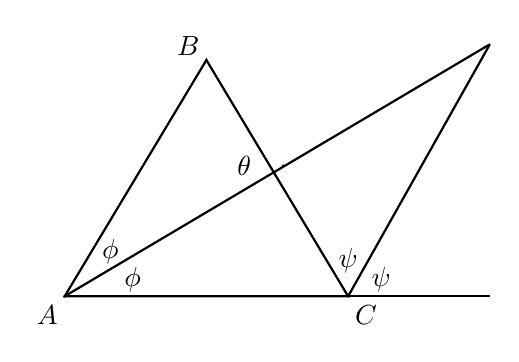
\begin{tikzpicture}
\coordinate (A) at (0,0 );
\coordinate (B) at (1.8,3);
\coordinate (C) at (3.6,0);
\coordinate (D) at (5.4,3.2);
\coordinate (E) at (2.775,1.66);


\filldraw[black] (A) circle (.2pt) node[anchor=south west, xshift=18, yshift=-2]{$\phi$};
\filldraw[black] (A) circle (.2pt) node[anchor= south west, xshift=10, yshift=8]{$\phi$};
\filldraw[black] (E) circle (.2pt) node[anchor=east, xshift=-8, yshift=0]{$\theta$};
\filldraw[black] (C) circle (.2pt) node[anchor=south, xshift=0, yshift=5]{$\psi$};
\filldraw[black] (C) circle (.2pt) node[anchor=south west, xshift=5, yshift=-2]{$\psi$};

\filldraw[black] (A) circle (.2pt) node[anchor=north  east , xshift=1, yshift=0]{$A$};
\filldraw[black] (B) circle (.2pt) node[anchor=south east, xshift=1, yshift=-2]{$B$};
\filldraw[black] (C) circle (.2pt) node[anchor=north west , xshift=-1,yshift=0]{$C$};

\draw[black,  thick] (A) -- (B) --( C) -- cycle;

\draw[black,  thick] (A)--(D);
\draw[black,  thick] (D) --  (C);
\draw[black,  thick] (5.4,0) --  (C);

\end{tikzpicture}
\newline


Homework 1.1.29
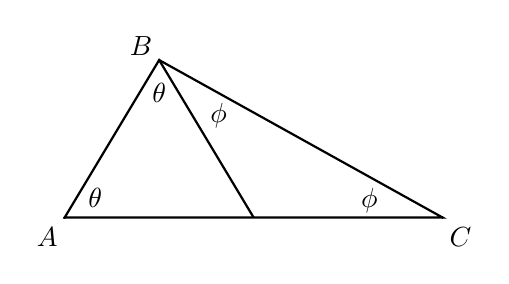
\begin{tikzpicture}
\coordinate (A) at (0,0 );
\coordinate (B) at (1.2,2);
\coordinate (C) at (4.8,0);
\coordinate (D) at (2.4,0);


\filldraw[black] (A) circle (.2pt) node[anchor=south west, xshift=5, yshift=0]{$\theta$};
\filldraw[black] (B) circle (.2pt) node[anchor= north, xshift=0, yshift=-5]{$\theta$};
\filldraw[black] (B) circle (.2pt) node[anchor=north west, xshift=15, yshift=-12]{$\phi$};
\filldraw[black] (C) circle (.2pt) node[anchor=south east, xshift=-20, yshift=-2]{$\phi$};

\filldraw[black] (A) circle (.2pt) node[anchor=north  east , xshift=1, yshift=0]{$A$};
\filldraw[black] (B) circle (.2pt) node[anchor=south east, xshift=1, yshift=-2]{$B$};
\filldraw[black] (C) circle (.2pt) node[anchor=north west , xshift=-1,yshift=0]{$C$};

\draw[black,  thick] (A) -- (B) --( C) -- cycle;

\draw[black,  thick] (B)--(D);

\end{tikzpicture}
\newline




Homework 1.1.30
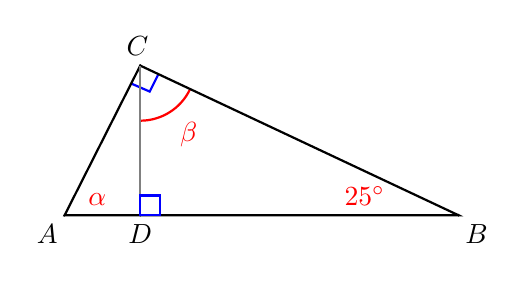
\begin{tikzpicture}
\coordinate (A) at (0,0 );
\coordinate (B) at (5,0);
\coordinate (C) at (.96,1.9);
\coordinate (D) at (.96,0);

\draw[red,thick] (.96,1.2) arc (270: 335:.7) node[below right, midway] {$\beta$};
\filldraw[black] (A) circle (.2pt) node[anchor=south west, xshift=5, yshift=0]{\color{red}$\alpha$};
\filldraw[black] (B) circle (.2pt) node[anchor= south east, xshift=-23, yshift=0]{\color{red}$25\degree$};

\filldraw[black] (A) circle (.2pt) node[anchor=north  east , xshift=1, yshift=0]{$A$};
\filldraw[black] (B) circle (.2pt) node[anchor=north west, xshift=-1, yshift=0]{$B$};
\filldraw[black] (C) circle (.2pt) node[anchor=south , xshift=-1,yshift=0]{$C$};
\filldraw[black] (D) circle (.2pt) node[anchor=north , xshift=0,yshift=0]{$D$};

\draw[blue,  thick] (0.85,1.67) -- (1.08,1.57) -- (1.19,1.79);
\draw[black,  thick] (A) -- (B) --( C) -- cycle;

\draw[gray,  thick] (C)--(D);
\draw[blue,  thick] (D) rectangle +(.25,.25);

\end{tikzpicture}
\newline


Homework 1.1.31
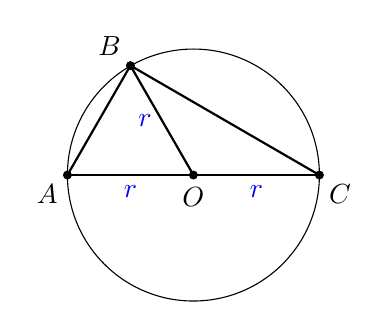
\begin{tikzpicture}
\coordinate(O) at (0,0);
\coordinate (A) at (-1.6,0 );
\coordinate (B) at (-0.8,1.39);
\coordinate (C) at(1.6,0);

\draw (0,0) circle (1.6);
\filldraw[black] (O) circle (1.4pt) node[anchor=north, xshift=0, yshift=-1]{$O$};
\filldraw[black] (A) circle (1.4pt) node[anchor=north east, xshift=0, yshift=0]{$A$};
\filldraw[black] (B) circle (1.4pt) node[anchor=south east, xshift=0, yshift=0]{$B$};
\filldraw[black] (C) circle (1.4pt) node[anchor=north west, xshift=0, yshift=0]{$C$};

\draw[black,  thick] (A) -- (B);
\draw[black,  thick] (B) --( C)  ;
\draw[black,  thick] (A) -- (O) node[below, midway]{\color{blue}$r$} ;
\draw[black, thick] (O) -- (C) node[below, midway]{\color{blue}$r$};
\draw[black,  thick] (B) --  (O) node[left, midway]{\color{blue}$r$};

\end{tikzpicture}
\newline



Homework 1.1.32
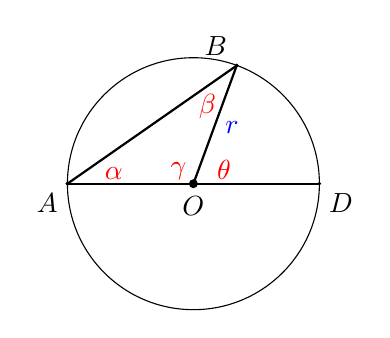
\begin{tikzpicture}
\coordinate(O) at (0,0);
\coordinate (A) at (-1.6,0 );
\coordinate (B) at (.55,1.5);
\coordinate (D) at(1.6,0);

\draw (0,0) circle (1.6);
\filldraw[black] (O) circle (1.4pt) node[anchor=north, xshift=0, yshift=-1]{$O$};
\filldraw[black] (O) circle (.4pt) node[anchor=south east, xshift=1, yshift=-2]{\color{red}$\gamma$};
\filldraw[black] (O) circle (.4pt) node[anchor=south west, xshift=5, yshift=-2]{\color{red}$\theta$};
\filldraw[black] (A) circle (.4pt) node[anchor=north east, xshift=0, yshift=0]{$A$};
\filldraw[black] (A) circle (.4pt) node[anchor=south west, xshift=10, yshift=-2]{\color{red}$\alpha$};
\filldraw[black] (B) circle (.4pt) node[anchor=south east, xshift=0, yshift=0]{$B$};
\filldraw[black] (B) circle (.4pt) node[anchor=north east, xshift=-4, yshift=-7]{\color{red}$\beta$};
\filldraw[black] (D) circle (.4pt) node[anchor=north west, xshift=0, yshift=0]{$D$};

\draw[black,  thick] (A) -- (B);
\draw[black,  thick] (A) -- (O) ;
\draw[black, thick] (O) -- (D) ;
\draw[black,  thick] (B) --  (O) node[right, midway, yshift=-1]{\color{blue}$r$};

\end{tikzpicture}
\newline



Homework 1.1.33
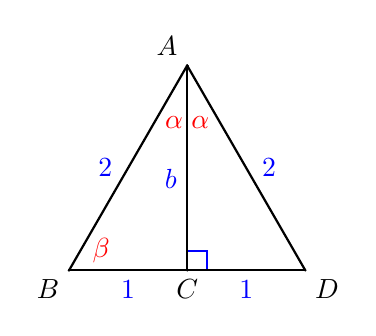
\begin{tikzpicture}
\coordinate (B) at (0,0 );
\coordinate (A) at (1.5,2.6);
\coordinate (C) at (1.5,0);
\coordinate (D) at (3,0);

\filldraw[black] (A) circle (.2pt) node[anchor=south  east , xshift=0, yshift=0]{$A$};
\filldraw[black] (A) circle (.2pt) node[anchor=north  east , xshift=2, yshift=-15]{\color{red}$\alpha$};
\filldraw[black] (A) circle (.2pt) node[anchor=north west , xshift=-2, yshift=-15]{\color{red}$\alpha$};
\filldraw[black] (B) circle (.2pt) node[anchor=north east, xshift=0, yshift=0]{$B$};
\filldraw[black] (B) circle (.2pt) node[anchor=south west, xshift=5, yshift=-1]{\color{red}$\beta$};
\filldraw[black] (C) circle (.2pt) node[anchor=north  , xshift=0,yshift=0]{$C$};
\filldraw[black] (D) circle (.2pt) node[anchor=north west, xshift=0, yshift=0]{$D$};

\draw[blue, thick] (C) rectangle +(0.25,0.25);
\draw[black,  thick] (A) -- (B) node[left, midway, xshift=-2]  {\color{blue}$2$};
\draw[black,  thick] (A) -- (D) node[right, midway, xshift=2]  {\color{blue}$2$};
\draw[black,  thick] (C) -- (B) node[below, midway]  {\color{blue}$1$};
\draw[black,  thick] (C) -- (D) node[below, midway]  {\color{blue}$1$};
\draw[black,  thick] (A)--(C) node [left, midway, yshift=-4] {\color{blue}$b$};

\end{tikzpicture}
\newline


Homework 1.1.34
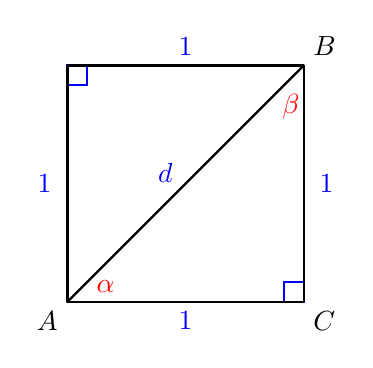
\begin{tikzpicture}
\coordinate (A) at (0,0 );
\coordinate (B) at (3,3);
\coordinate (C) at (3,0);
\coordinate (D) at (0,3);

\filldraw[black] (A) circle (.2pt) node[anchor=north  east , xshift=0, yshift=0]{$A$};
\filldraw[black] (A) circle (.2pt) node[anchor=south west , xshift=7, yshift=0]{\color{red}$\alpha$};
\filldraw[black] (B) circle (.2pt) node[anchor=south west, xshift=0, yshift=0]{$B$};
\filldraw[black] (B) circle (.2pt) node[anchor=north east, xshift=2, yshift=-7]{\color{red}$\beta$};
\filldraw[black] (C) circle (.2pt) node[anchor=north  west, xshift=0,yshift=0]{$C$};

\draw[blue, thick] (C) rectangle +(-0.25,0.25);
\draw[blue, thick] (D) rectangle +(0.25,-0.25);
\draw[black,  thick] (A) -- (B) node[left, midway, xshift=-1, yshift=4]  {\color{blue}$d$};
\draw[black,  thick] (A) -- (D) node[left, midway, xshift=-2]  {\color{blue}$1$};
\draw[black,  thick] (C) -- (B) node[right, midway, xshift=2]  {\color{blue}$1$};
\draw[black,  thick] (B) -- (D) node[above, midway]  {\color{blue}$1$};
\draw[black,  thick] (A)--(C) node [below, midway] {\color{blue}$1$};

\end{tikzpicture}
\newline



Homework 1.1.35
\begin{tikzpicture}
\coordinate (A) at (0,0 );
\coordinate (B) at (1.2,0);
\coordinate (C) at (0,1);
\coordinate (D) at (2,1);

\filldraw[black] (D) circle (.2pt) node[anchor=south  west , xshift=8, yshift=0]{\color{red}$47\degree$};
\filldraw[black] (D) circle (.2pt) node[anchor=north  east , xshift=-6, yshift=0]{\color{red}$x$};
\filldraw[black] (B) circle (.2pt) node[anchor=north, xshift=4, yshift=0]{\color{red}$y$};

\draw[black,  thick] (-.5,0) -- (3.2,0) ;
\draw[black,  thick, <-] (A) -- (B) ;
\draw[black,  thick] (.8,-.5) -- (2.4,1.5) ;
\draw[black,  thick] (-.5,1) -- (3.2,1) ;
\draw[black,  thick, <-] (C) -- (D) ;

\end{tikzpicture}
\newline



Homework 1.1.36
\begin{tikzpicture}
\coordinate (A) at (0,0 );
\coordinate (B) at (-1.8,1);
\coordinate (C) at (1.8,-1);

\filldraw[black] (A) circle (.2pt) node[anchor=south  east , xshift=0, yshift=5]{\color{red}$x$};
\filldraw[black] (A) circle (.2pt) node[anchor=north  east , xshift=0, yshift=0]{\color{red}$y$};
\filldraw[black] (A) circle (.2pt) node[anchor=north west, xshift=20, yshift=0]{\color{red}$28\degree$};

\draw[blue, thick] (A) rectangle +(.25,.25);
\draw[black,  thick] (A) -- (2,0) ;
\draw[black,  thick] (0,-1) -- (0,1) ;
\draw[black,  thick] (B) -- (C) ;

\end{tikzpicture}
\newline



Homework 1.1.37
\begin{tikzpicture}
\coordinate (A) at (0,0 );
\coordinate (B) at (1.8,.9);
\coordinate (C) at (B)++(-1,.5);
\coordinate (D) at (-1,-.5 );
\coordinate (E) at (B)++(-1,2);

\filldraw[black] (A) circle (.2pt) node[anchor=south   , xshift=0, yshift=11]{\color{red}$2x+30$};
\filldraw[black] (A) circle (.2pt) node[anchor=west , xshift=9, yshift=-2]{\color{red}$x-2y$};
\filldraw[black] (B) circle (.2pt) node[anchor=north , xshift=0, yshift=-5]{\color{red}$150\degree$};

\draw[black,  thick] (-2.5,1.25) -- +(4,-2) ;
\draw[black,  thick] (D) -- +(4,2) ;
\draw[black,  thick] (B)++(1.4,-.7) -- +(-5,2.5) ;
\draw[black,  thick, ->] (A) -- +(-1.6,.8);
\draw[black,  thick, ->] (B) --+ (-2.6,1.3) ;

\draw[red, thick] (.36,.18) arc (26.6:153.4:.4);
\draw[red, thick] (1.6,.79) arc (206.6:333.4:.25);
\draw[red, thick] (.27,.134) arc (26.6:-26.6:.3);

\end{tikzpicture}
\newline




Homework 1.1.38
\begin{tikzpicture}
\coordinate (A) at (0,0 );
\coordinate (B) at (2,.728);
\coordinate (C) at (A)++(0,2);
\coordinate (D) at (2,2);

\draw[black,  thick] (-1.5,-.546) -- +(4.5,1.638) ;
\draw[black,  thick] (0,-1) -- +(0,3.5) ;
\draw[black,  thick] (2,-1) -- +(0,3.5) ;
\draw[black,  thick, ->] (A) -- +(0,2);
\draw[black,  thick, ->] (B) -- (2,2) ;

\draw[red, thick] (0,-.4) arc (-90:-160:.4) node[below left, midway, yshift=-3] {$x+2y$};
\draw[red, thick] (0,-.25) arc (-90:20:.25) node [below right] {$3x-10$};
\draw[red, thick] (2,.428) arc (-90:20:.3) node [below right] {$110\degree$};

\end{tikzpicture}
\newline



Homework 1.1.39
\begin{tikzpicture}
\coordinate (A) at (0,0 );

\draw[black,  thick] (0.13,-.75) -- (-.397,2.25) ;
\draw[black,  thick] (-2,0) -- +(4,0) ;
\draw[black,  thick] (-2,1.5) -- +(4,0) ;
\draw[black,  thick, ->] (A) -- +(1.5,0);
\draw[black,  thick, ->] (0,1.5) -- +(1.5,0) ;

\draw[red, thick] (.3,0) arc (0:-80:.3) node[below right, midway, yshift=2] {$4x-20y$};
\draw[red, thick] (-.3,0) arc (180:100:.3) node [above left, xshift=-5,yshift=-5] {$3y+32$};
\draw[red, thick] (.041,1.5) arc (0:-80:.35) node [below right, xshift=3,yshift=3] {$5y$};

\end{tikzpicture}
\newline

Homework 1.1.40
\begin{tikzpicture}
\coordinate (A) at (0,0 );
\coordinate (B) at (0,1);
\coordinate (C) at(-2,-.5);
\coordinate (D) at(2,.5);
\coordinate (E) at (-2,.5);
\coordinate (F) at (2,1.5);

\draw[black,  thick] (0.,-1.) -- +(0,3) ;
\draw[black,  thick, ->] (C) -- (D) ;
\draw[black,  thick, ->] (E) -- (F) ;
\draw[black,  thick] (D) -- +(.5,.125);
\draw[black,  thick] (F) --+ (.5,.125) ;

\draw[red, thick] (0,.3) arc (90:194:.3) node[left, midway] {$100\degree$};
\draw[red, thick] (0,-.3) arc (270:374:.3) node[right, midway, yshift=-4] {$x+3y$};
\draw[red, thick] (0,1.3) arc (90:14:.3) node[right, midway, xshift=-7, yshift=8] {$2x+2y$};

\end{tikzpicture}
\newline



Homework 1.1.41
\begin{tikzpicture}
\coordinate (A) at (0,0 );
\coordinate (B) at (0.7,-1);
\coordinate (C) at(1.36,1.94);
\coordinate (D) at(1.15,1.64);
\coordinate (E) at (3.5,0);
\coordinate (F) at (-1,-1.43);
\coordinate (G) at (-.638,-.9116);
\coordinate (H) at (-1.94,0);

\draw[blue,thick] (G)++(-.164,.115) -- ++(.115,.164) -- +(.164,-.115);

\draw[black,  thick] (-2.5,0) -- (E) ;
\draw[black,  thick] (E) -- (D) ;
\draw[black,  thick] (C) -- (F) ;
\draw[black,  thick] (.056,-1.4116) -- (H);
\draw[black,  thick, ->] (E) --+ (-1.5,1.05) ;
\draw[black,  thick, ->] (G) --+ (-.5,.35) ;

\filldraw[black] (D) circle (.2pt) node[anchor=west, xshift=3]{\color{red}$x$};
\filldraw[black] (A) circle (.2pt) node[anchor=north east, xshift=-6]{\color{red}$y$};
\filldraw[black] (E) circle (.2pt) node[anchor=south east, xshift=-12,yshift=-1]{\color{red}$35\degree$};

\end{tikzpicture}
\newline



Homework 1.1.42
\begin{tikzpicture}
\coordinate (A) at (0,0 );
\coordinate (B) at (2.5,0);
\coordinate (C) at(.44,2.5);

\draw[black,  thick] (A) -- (B) --(C) -- cycle;
\draw[black,  thick] (-1.,0) -- (3.5,0) ;
\draw[black,  thick] (-1.,2.5) -- (3.5,2.5) ;
\draw[black,  thick, ->] (A) -- (3,0) ;
\draw[black,  thick, ->] (C) -- (3.0,2.5) ;

\filldraw[black] (C) circle (.2pt) node[anchor=north west, xshift=7]{\color{red}$x$};
\filldraw[black] (C) circle (.2pt) node[anchor=north, xshift=3,yshift=-9]{\color{red}$x$};
\filldraw[black] (A) circle (.2pt) node[anchor=south west, xshift=0,yshift=0]{\color{red}$80\degree$};
\filldraw[black] (B) circle (.2pt) node[anchor=south west, xshift=-1,yshift=-1]{\color{red}$y$};

\end{tikzpicture}
\newline



Homework 1.1.43
\begin{tikzpicture}
\coordinate (A) at (0,0 );
\coordinate (B) at (2.5,0);
\coordinate (C) at(.44,2.5);

\draw[black,  thick] (A) -- (B) --(C) -- cycle;
\draw[black,  thick] (-1.,0) -- (3.5,0) ;
\draw[black,  thick] (-1.,2.5) -- (3.5,2.5) ;
\draw[black,  thick, ->] (A) -- (3,0) ;
\draw[black,  thick, ->] (C) -- (3.0,2.5) ;

\filldraw[black] (C) circle (.2pt) node[anchor=north east, xshift=0]{\color{red}$y$};
\filldraw[black] (A) circle (.2pt) node[anchor=south east, xshift=1,yshift=0]{\color{red}$100\degree$};
\filldraw[black] (B) circle (.2pt) node[anchor=south east, xshift=-6,yshift=-1]{\color{red}$x$};
\node at (1.25,-.3) {\color{blue}$6$};
\node at (0,1.25) {\color{blue}$6$};

\end{tikzpicture}
\newline



Homework 1.1.44
\begin{tikzpicture}
\coordinate (A) at (0,0 );
\coordinate (B) at (2.7,1.25);
\coordinate (C) at(0,2.5);

\draw[black,  thick] (A) -- (B) --(C) -- cycle;
%\draw[black,  thick] (-1.,0) -- (3.5,0) ;
\draw[black,  thick] (B) -- (2.7,2.5) ;
\draw[black,  thick] (-.91,-.43) -- (3.61,1.68) ;
\draw[black,  thick, ->] (A) -- +(0,1.25) ;
\draw[black,  thick, ->] (B) -- +(0,1) ;

\filldraw[black] (C) circle (.2pt) node[anchor=north west, xshift=-1, yshift=-9]{\color{red}$65\degree$};
\filldraw[black] (B) circle (.2pt) node[anchor=south west, xshift=0,yshift=1]{\color{red}$y$};
\filldraw[black] (B) circle (.2pt) node[anchor=south east, xshift=0,yshift=2]{\color{red}$x$};
\node at (1.35,2.2) {\color{blue}$15$};
\node at (1.35,.3) {\color{blue}$15$};

\end{tikzpicture}
\newline



Homework 1.1.45
\begin{tikzpicture}
\coordinate (A) at (0,0 );
\coordinate (B) at (3,0);
\coordinate (C) at(2.5,2);

\draw[black,  thick] (A) -- (B) --(C) -- cycle;
\draw[black,  thick] (-.5,0) -- (5,0) ;
\draw[black,  thick] (-.5,2) -- (5,2) ;
\draw[black,  thick, ->] (A) -- (4,0) ;
\draw[black,  thick, ->] (0,2) -- (4,2) ;

\filldraw[black] (C) circle (.2pt) node[anchor=north east, xshift=-14, yshift=0]{\color{red}$4$};
\filldraw[black] (C) circle (.2pt) node[anchor=north , xshift=-3, yshift=-5]{\color{red}$2$};
\filldraw[black] (C) circle (.2pt) node[anchor=north west, xshift=2, yshift=0]{\color{red}$5$};
\filldraw[black] (A) circle (.2pt) node[anchor=south west, xshift=12,yshift=-1]{\color{red}$1$};
\filldraw[black] (B) circle (.2pt) node[anchor=south east, xshift=-1,yshift=-1]{\color{red}$3$};

\end{tikzpicture}
\newline



Homework 1.1.46a
\begin{tikzpicture}
\coordinate (A) at (0,0 );
\coordinate (B) at (4.5,0);
\coordinate (C) at(3.45,1.68);
\coordinate (D) at(5,2.43);

\draw[black,  thick, dashed] (A) -- (C) ;
\draw[black,  thick] (C) -- (D) ;
\draw[black,  thick] (B) -- (C) ;
\draw[black,  thick] (5.4,0) -- +(.5,0) ;
\draw[black,  thick] (5.4,2.43) -- +(.5,0) ;
\draw[black,  thick, ->] (A) -- (5.4,0) ;
\draw[black,  thick, ->] (0,2.43) -- (5.4,2.43) ;

\filldraw[black] (D) circle (.2pt) node[anchor=north east, xshift=-20, yshift=0]{\color{red}$26\degree$};
\filldraw[black] (C) circle (.2pt) node[anchor=west , xshift=7, yshift=-1]{\color{red}$\theta$};
\filldraw[black] (B) circle (.2pt) node[anchor=south east, xshift=-5,yshift=-1]{\color{red}$58\degree$};

\end{tikzpicture}
\newline



Homework 1.1.46b
\begin{tikzpicture}
%\coordinate (A) at (0,0 );
\coordinate (B) at (3.5,0);
\coordinate (C) at(2,.8);
\coordinate (D) at(3.2,2.4);

\draw[black,  thick] (C) -- (D) ;
\draw[black,  thick] (B) -- (C) ;
\draw[black,  thick] (0,0) -- (5,0) ;
\draw[black,  thick] (0,2.4) -- +(5,0) ;
\draw[black,  thick, ->] (0,0) -- (4,0) ;
\draw[black,  thick, ->] (0,2.4) -- (4,2.4) ;

\filldraw[black] (D) circle (.2pt) node[anchor=north east, xshift=-7, yshift=0]{\color{red}$v$};
\filldraw[black] (C) circle (.2pt) node[anchor=west , xshift=6, yshift=1]{\color{red}$\theta$};
\filldraw[black] (B) circle (.2pt) node[anchor=south east, xshift=-18,yshift=-1]{\color{red}$w$};

\end{tikzpicture}
\newline


Homework 1.1.47
\begin{tikzpicture}
\coordinate (A) at (0,0 );
\coordinate (B) at (2.5,0);
\coordinate (C) at(2.5,-5);
\coordinate (D) at(0,-5);
\coordinate (Q) at (1.25,-2.5);

\draw[black,  thick] (A) rectangle (C) ;
\draw[black,  thin] (B) -- (D) ;
\draw[black,  thin] (A) -- (C) ;

\filldraw[black] (B) circle (.2pt) node[anchor=north east, xshift=-7, yshift=0]{\color{red}$4$};
\filldraw[black] (B) circle (.2pt) node[anchor=north east, xshift=1, yshift=-16]{\color{red}$5$};
\filldraw[black] (D) circle (.2pt) node[anchor=south west , xshift=4, yshift=0]{\color{red}$3$};
\filldraw[black] (Q) circle (2pt) node[anchor=south, xshift=0,yshift=6]{$Q$};
\filldraw[black] (Q) circle (1.5pt) node[anchor=east, xshift=0,yshift=0]{\color{red}$130\degree$};
\filldraw[black] (Q) circle (.8pt) node[anchor=west, xshift=2,yshift=0]{\color{red}$1$};
\filldraw[black] (Q) circle (.8pt) node[anchor=north, xshift=0,yshift=-6]{\color{red}$2$};
\filldraw[black] (A) circle (.8pt) node[anchor=south east, xshift=0,yshift=0]{$A$};
\filldraw[black] (B) circle (.8pt) node[anchor=south west, xshift=0,yshift=0]{$B$};
\filldraw[black] (C) circle (.8pt) node[anchor=north west, xshift=0,yshift=0]{$C$};
\filldraw[black] (D) circle (.8pt) node[anchor=north east, xshift=0,yshift=0]{$D$};

\end{tikzpicture}
\newline



Homework 1.1.48
\begin{tikzpicture}
\coordinate (O) at (0,0 );
\coordinate (A) at (0.174,1.99 ); %80 degree
\coordinate (B) at (0.845,-1.813); %-65 deg
\coordinate (C) at(6.579,.8606);

\draw (O) circle (2);
\draw[black,  thick] (A) -- (C) ;
\draw[black,  thick] (B) -- (C) ;
\draw[black,  thick] (A) -- (B) ;
\draw[black,  thick] (A) -- (O) ;
\draw[black,  thick] (O) -- (B) ;
\draw[black,  thick] (O) -- (C) ;

\filldraw[black] (O) circle (1.5pt) node[anchor=east, xshift=0,yshift=0]{$O$};
\filldraw[black] (A) circle (.2pt) node[anchor=south, xshift=0,yshift=0]{$A$};
\filldraw[black] (B) circle (.2pt) node[anchor=north , xshift=0, yshift=0]{$B$};
\filldraw[black] (C) circle (.2pt) node[anchor=west, xshift=1, yshift=0]{$C$};

\filldraw[black] (O) circle (1.5pt) node[anchor=south west, xshift=-1,yshift=-1]{\color{red}$5$};
\filldraw[black] (A) circle (1.5pt) node[anchor=north, xshift=1,yshift=-22]{\color{red}$1$};
\filldraw[black] (A) circle (1.5pt) node[anchor=north west, xshift=0,yshift=0]{\color{red}$2$};
\filldraw[black] (C) circle (1.5pt) node[anchor=east, xshift=-30,yshift=0]{\color{red}$3$};
\node at (.7,.3) {\color{red}$4$};


\end{tikzpicture}
\newline






Exercise not used?
\begin{tikzpicture}
\coordinate (O) at (0,0);
\coordinate (A) at (0,0);
\coordinate (B) at (0,0);
\coordinate(C) at (0,0);
\coordinate (D) at (0,0);
\filldraw[black] (O) circle (.2pt) node[anchor=south west, xshift=6]{$50\degree$};
\filldraw[black] (A) circle (.2pt) node[anchor=south east]{$x$};
\filldraw[black] (B) circle (.2pt) node[anchor=north east, xshift=-6]{$y$};
\filldraw[black] (C) circle (.2pt) node[anchor=north west]{$z$};
%\draw[black,  thick] (A) -- (B) --( C) -- cycle;
\draw[black] (-2.3,0) --  (2.3,0);
\draw[black] (0.8,1.3) --  (-0.8,-1.3) ;
\end{tikzpicture}
\newline


\end{document}
